\chapter{Performance Evaluation}
\label{cha:evaluation}
\vspace{0.4 cm}

In this chapter, the proposed system is validated and the performance of the models for the different use cases is evaluated.
The first section presents the datasets provided by MIWEnergia.
Subsequently, the adapted evaluation methodology is described.
Finally, the evaluation of the performance of the models for the different use cases is presented.
After this chapter, it will be clear how the system has been validated and what the performance achieved by the proposed system is.


\section{MIWEnergia datasets}
\label{sec:datasets}
\vspace{0.2 cm}

Describe the MIWEnergia\footnote{ \url{https://www.miwenergia.com/} } datasets ...

Report plots of the data ...

Aggregated consumption data on all customers, whose number is variable (maximum 4253, minimum 1591, mean 2988): from June 2021 to September 2022 (January 2023), hourly aggregated data, 11687 (14617) total entries.
The graphical representation of the hourly aggregated consumption data is reported in figure~\ref{fig:demanddataplot}. (Include also plot with latest data)

\begin{figure}[H]
\centering
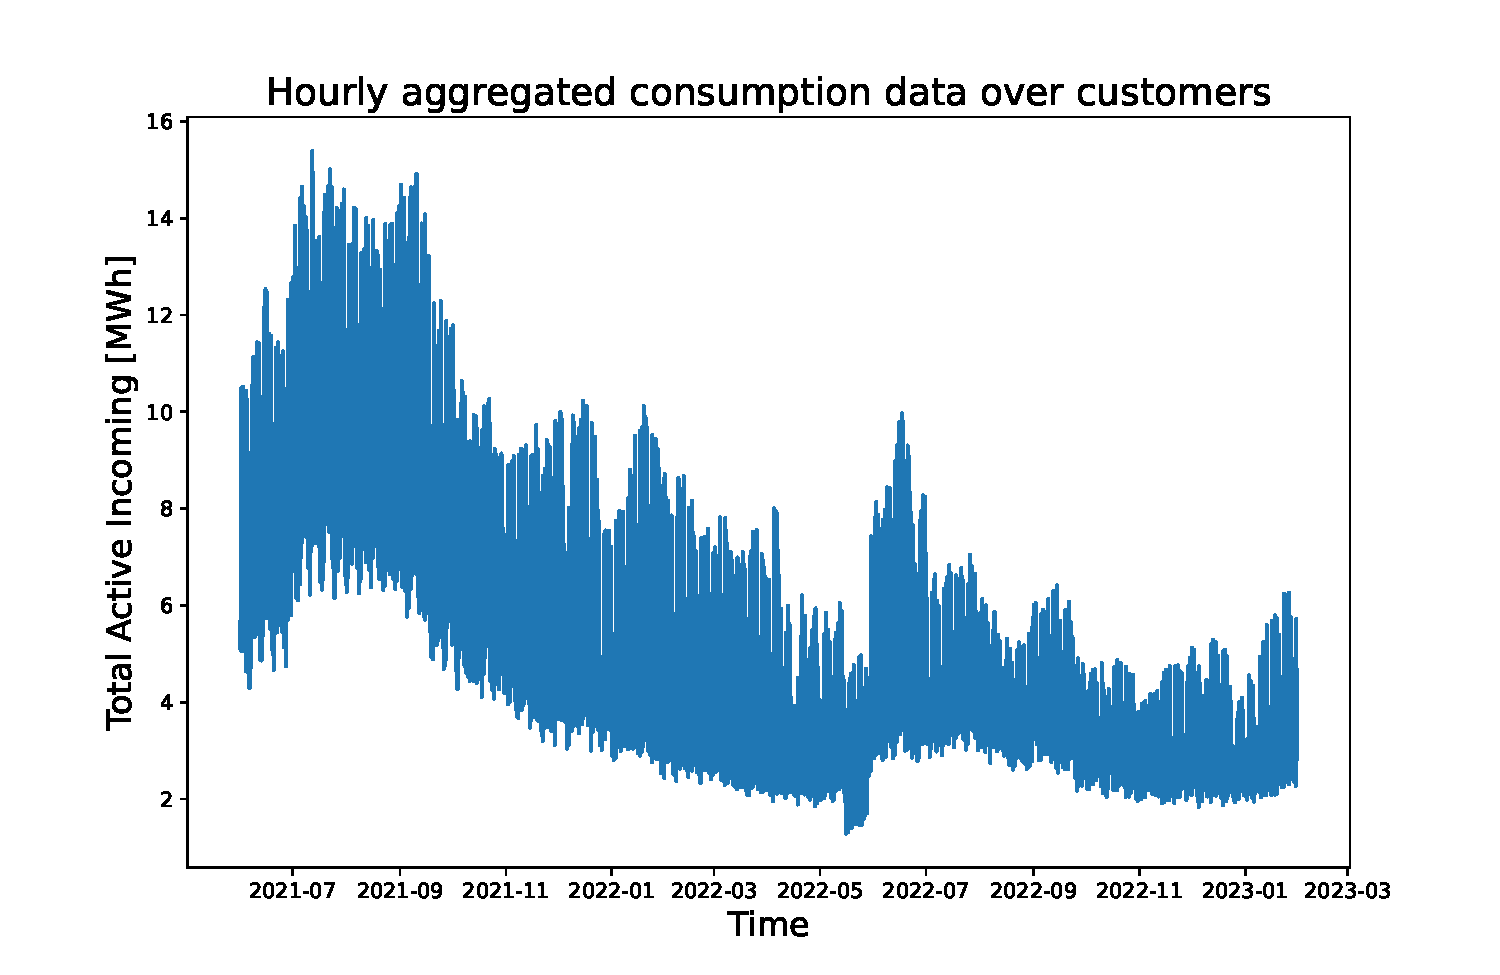
\includegraphics[width=0.6\textwidth]{images/demand/data_plot}
\caption{The graphical representation of the hourly aggregated consumption data.}
\label{fig:demanddataplot}
\end{figure}


Consumption data of 4 customers:
\begin{enumerate}
  \item from June 2021 to May 2022, hourly aggregated, 8750 total entries (represented in figure~\ref{fig:dataplotcustomer1});
  \item from September 2021 to May 2022, hourly aggregated, 5855 total entries (represented in figure~\ref{fig:dataplotcustomer2});
  \item from September 2021 to August 2022, hourly aggregated, 8745 total entries (represented in figure~\ref{fig:dataplotcustomer3}).
  \item from September 2021 to August 2022, hourly aggregated, 8760 total entries (represented in figure~\ref{fig:dataplotcustomer4});
\end{enumerate}
Total: from June 2021 to August 2022, hourly aggregated, 32110 total entries.

\begin{figure}[H]
\begin{minipage}[b]{8.5cm}
\centering
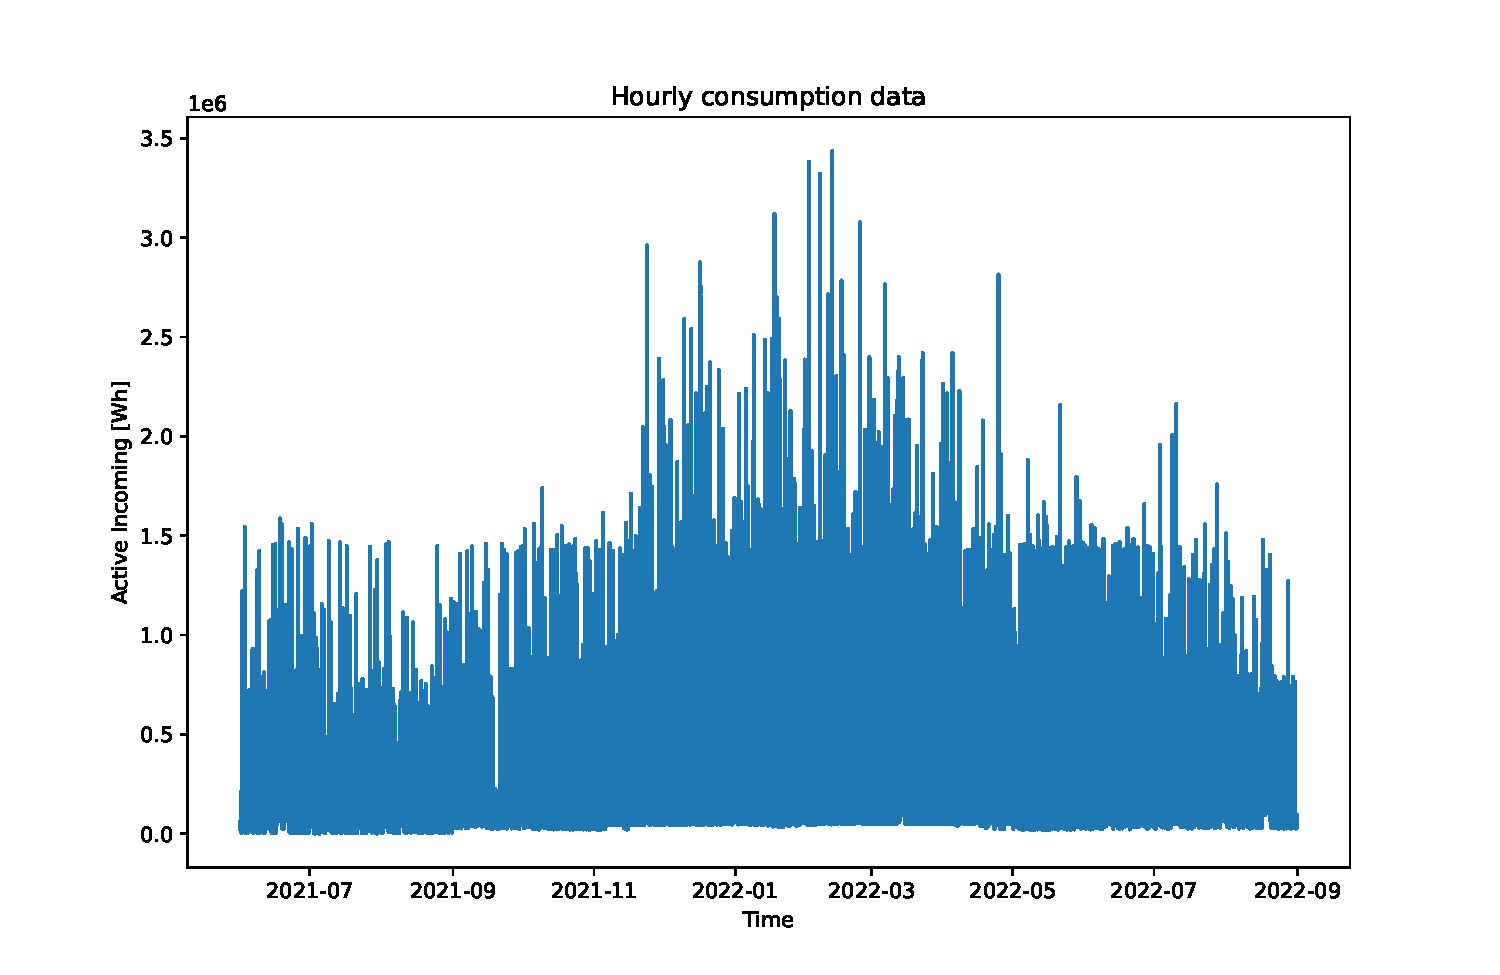
\includegraphics[width=0.9\textwidth]{images/baseline/data_plot_customer1}
\subcaption{First customer.}
\label{fig:dataplotcustomer1}
\end{minipage}
\ \hspace{2mm} \
\begin{minipage}[b]{8.5cm}
\centering
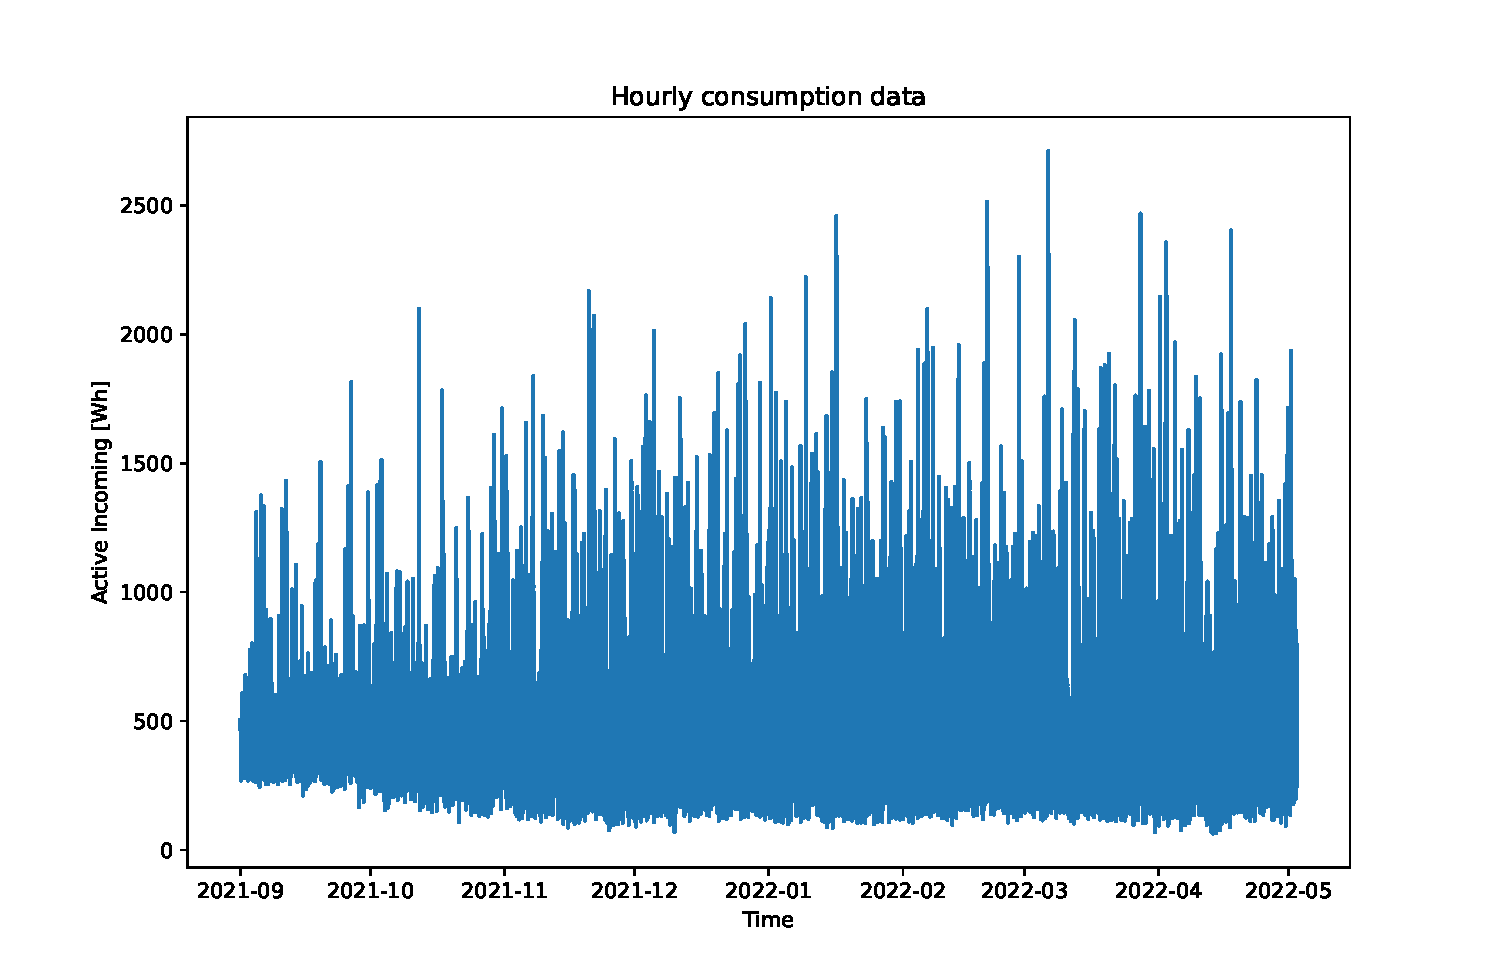
\includegraphics[width=0.9\textwidth]{images/baseline/data_plot_customer2}
\subcaption{Second customer.}
\label{fig:dataplotcustomer2}
\end{minipage}
\begin{minipage}[b]{8.5cm}
\centering
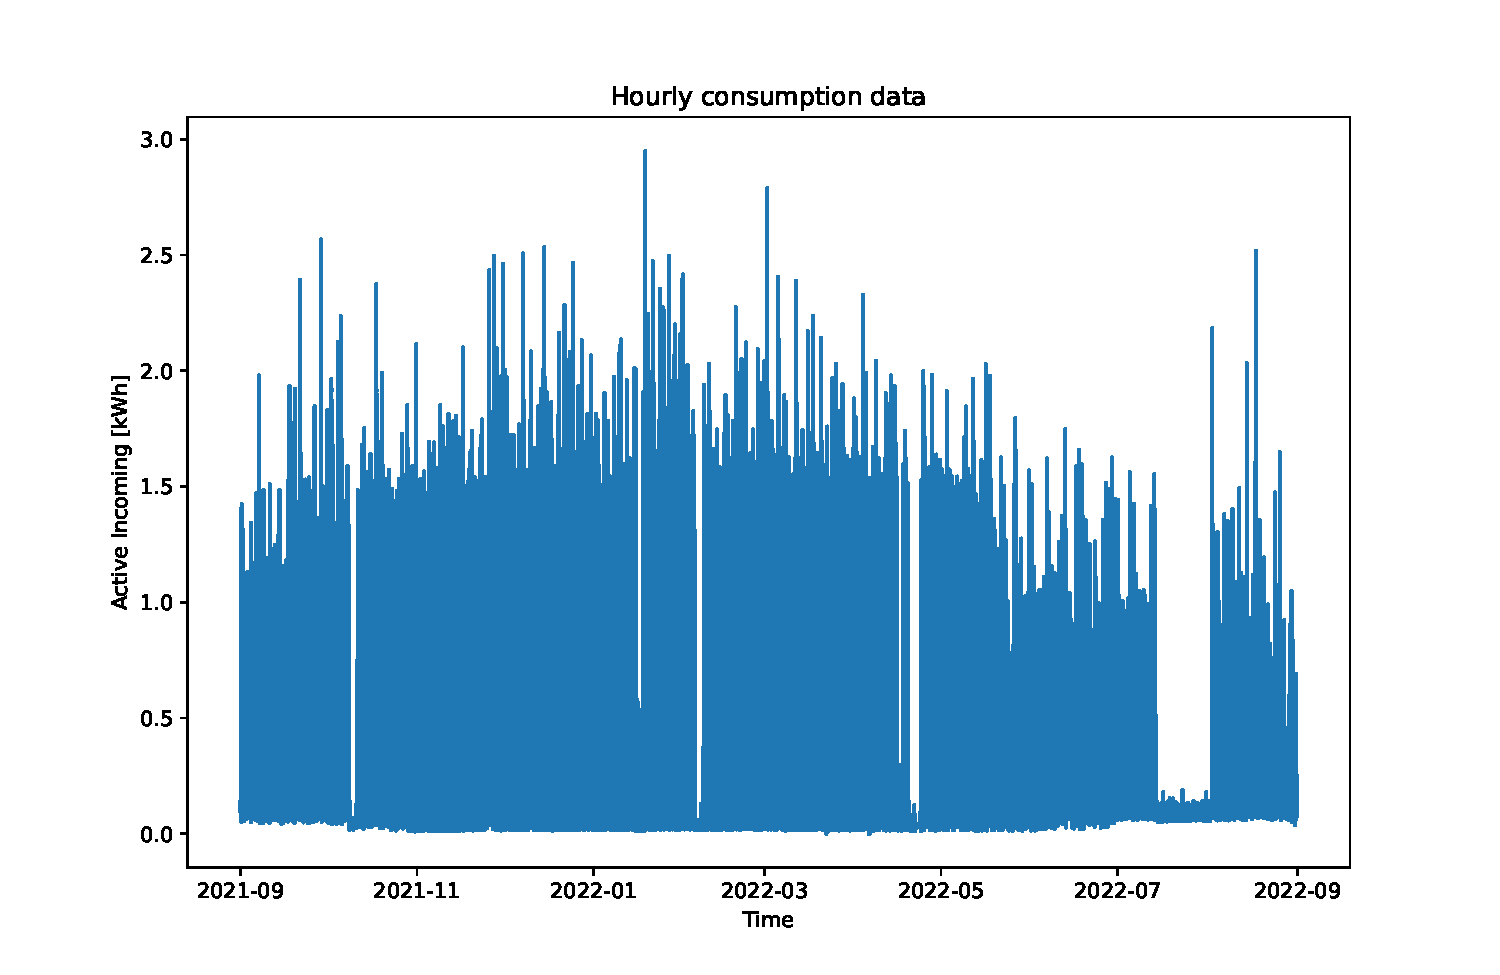
\includegraphics[width=0.9\textwidth]{images/baseline/data_plot_customer3}
\subcaption{Third customer.}
\label{fig:dataplotcustomer3}
\end{minipage}
\ \hspace{2mm} \
\begin{minipage}[b]{8.5cm}
\centering
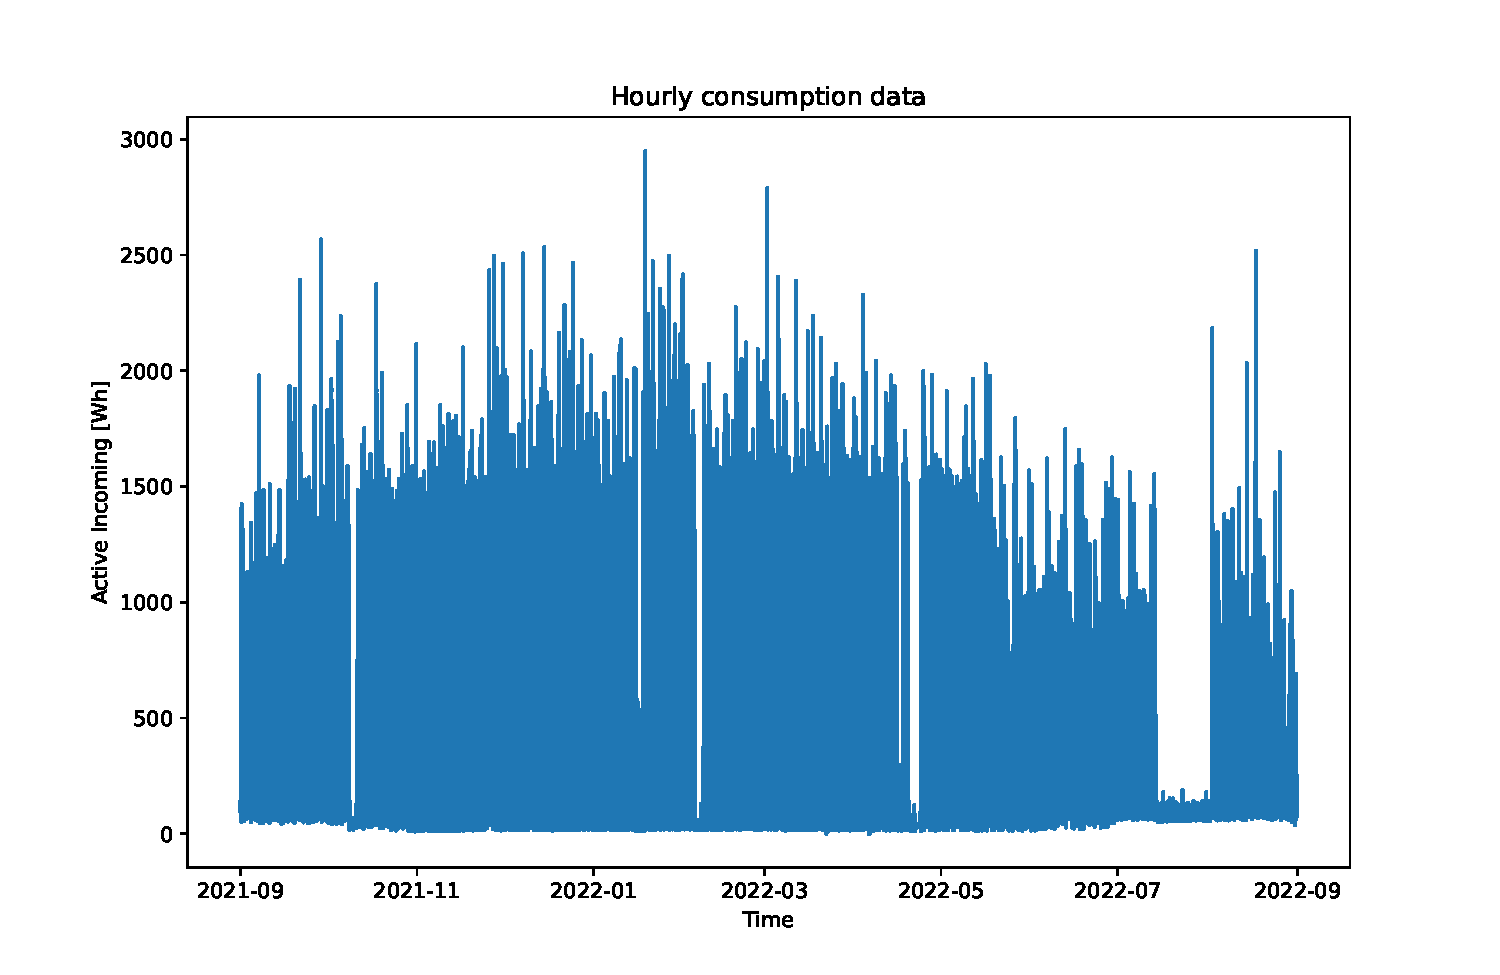
\includegraphics[width=0.9\textwidth]{images/baseline/data_plot_customer4}
\subcaption{Fourth customer.}
\label{fig:dataplotcustomer4}
\end{minipage}
\caption{The graphical representation of the consumption data of the 4 customers.}
\end{figure}

Production data of 8 plants:
\begin{enumerate}
  \item from January 2022 to October 2022, hourly aggregated, 7296 total entries;
  \item from February 2022 to October 2022, hourly aggregated, 6552 total entries;
  \item from February 2022 to October 2022, hourly aggregated, 6552 total entries;
  \item from June 2022 to October 2022, hourly aggregated, 3576 total entries;
  \item from September 2022 to October 2022, hourly aggregated, 1465 total entries;
  \item from September 2022 to October 2022, hourly aggregated, 1465 total entries;
  \item from September 2022 to October 2022, hourly aggregated, 1465 total entries;
  \item from September 2022 to October 2022, hourly aggregated, 1465 total entries.
\end{enumerate}
Total: from January 2022 to October 2022, hourly aggregated, 29836 total entries.
The graphical representation of the hourly aggregated total and mean percentage production data are reported respectively in figure~\ref{fig:productiondataplot} and figure~\ref{fig:productiondataplotpercentage}.

\begin{figure}[H]
\begin{minipage}[b]{8.5cm}
\centering
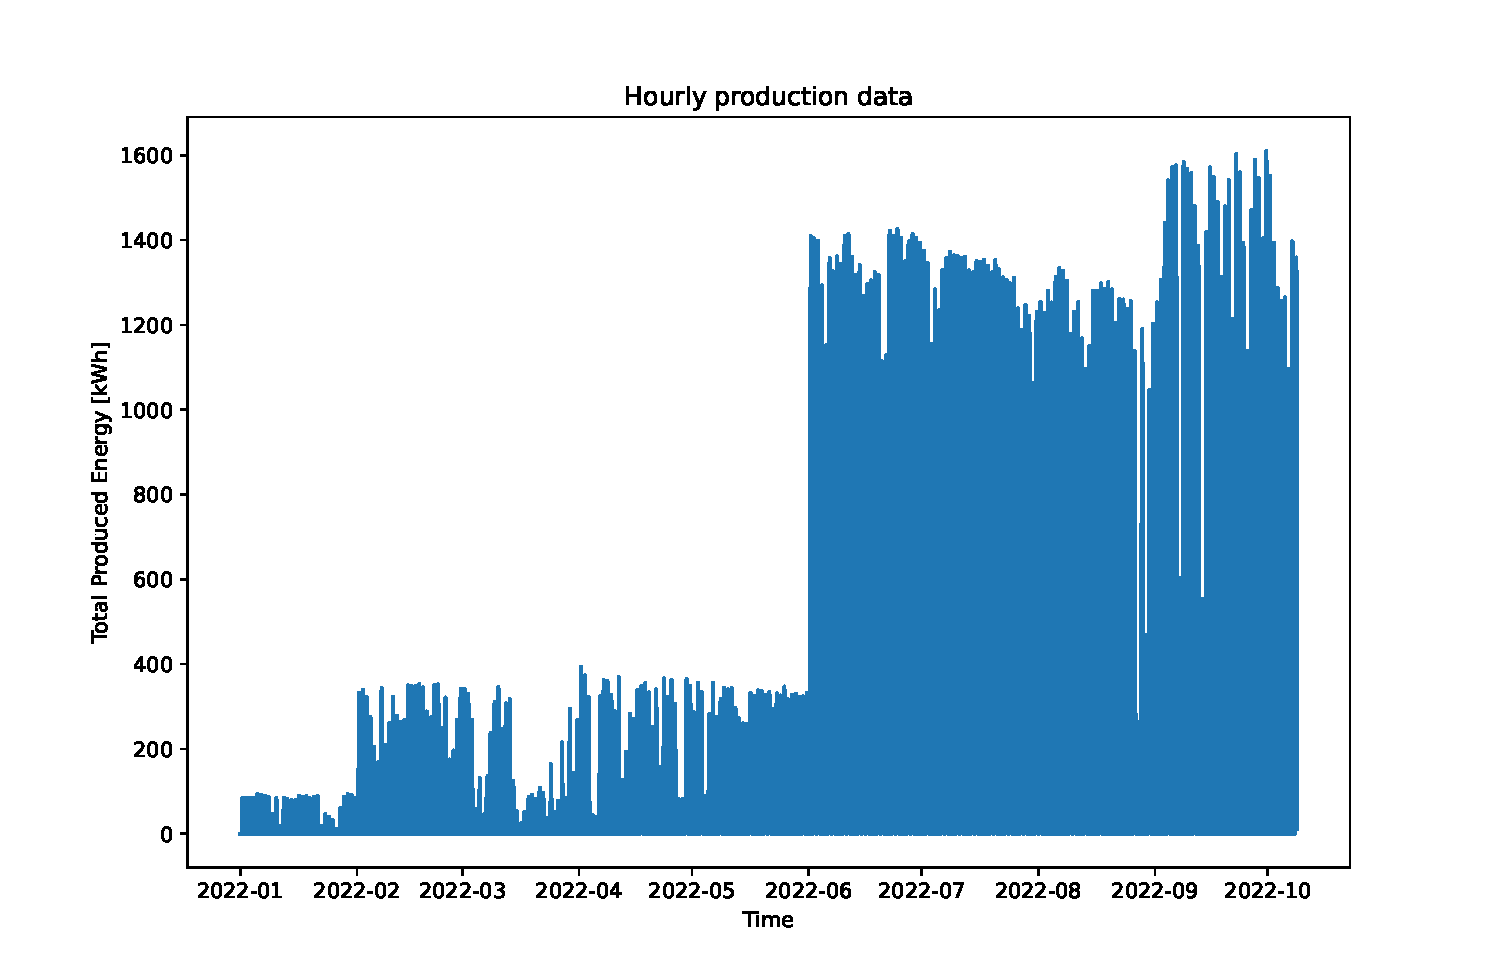
\includegraphics[width=0.9\textwidth]{images/production/data_plot}
\subcaption{}
\label{fig:productiondataplot}
\end{minipage}
\ \hspace{2mm} \
\begin{minipage}[b]{8.5cm}
\centering
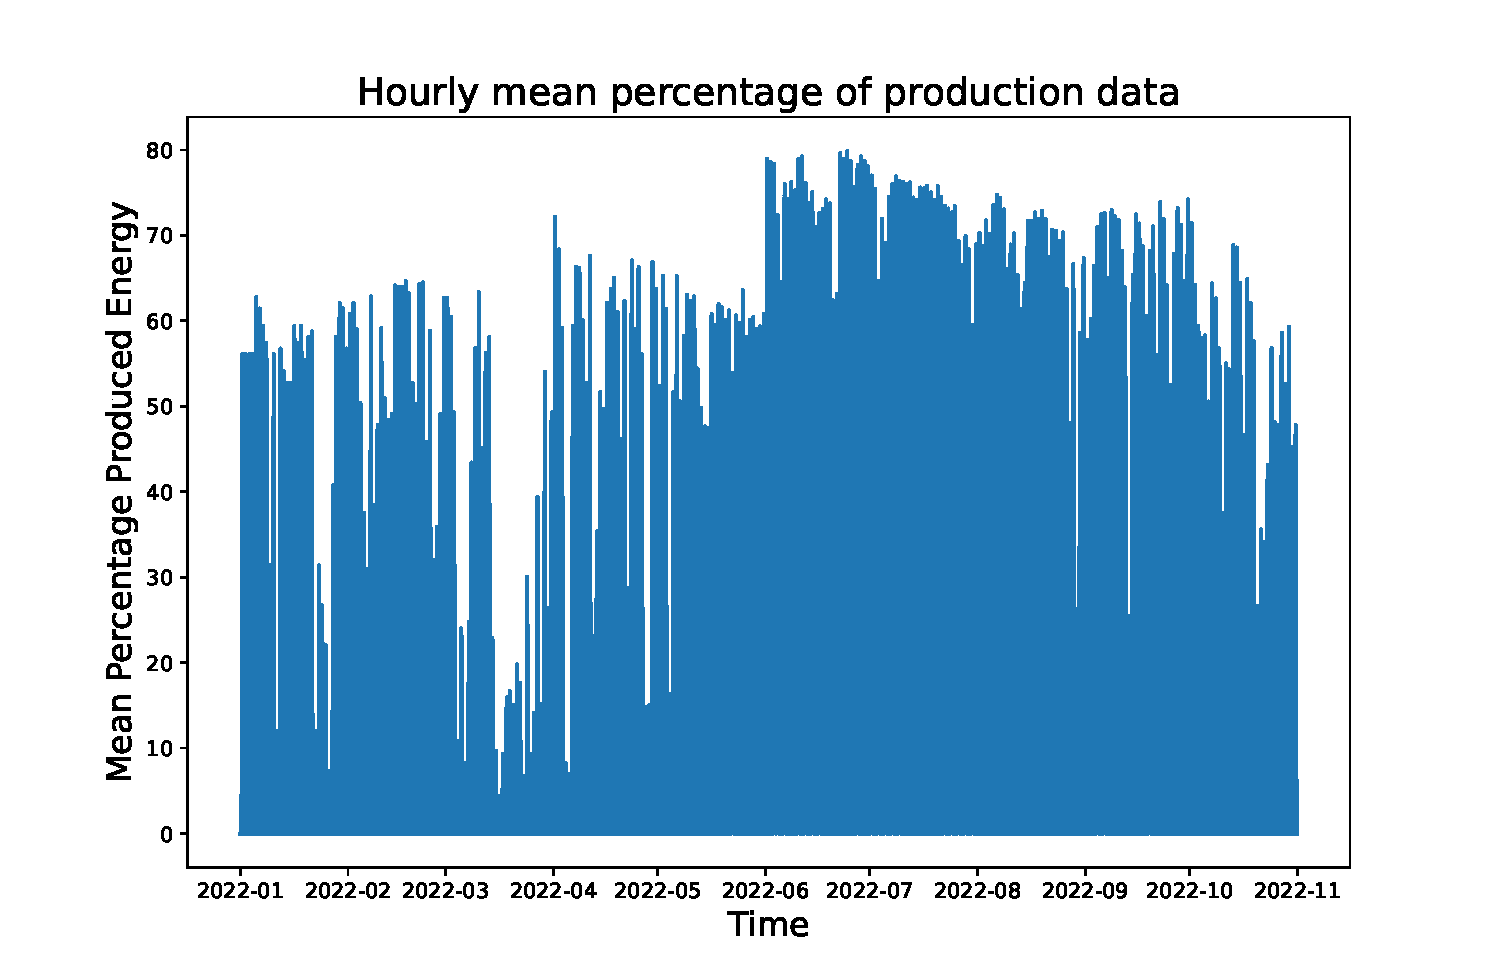
\includegraphics[width=0.9\textwidth]{images/production/data_plot_percentage}
\subcaption{}
\label{fig:productiondataplotpercentage}
\end{minipage}
\caption{The graphical representation of the hourly aggregated \subref{fig:umlsingleplant} total and \subref{fig:umlsingleplant} mean percentage production data.}
\end{figure}


\section{Evaluation methodology}
\label{sec:methodology}
\vspace{0.2 cm}

General description of the evaluation methodology ...

Describe the relevant error metrics:

Mean Absolute Percentage Error (MAPE) is defined as … (it is the most relevant error metric for all the tasks)

Mean Absolute Error (MAE) is defined as … (it is most applicable in Consumption baseline forecasting (where there is a high variability) and Electricity production forecasting (where there are a lot of zeros))

Describe how the test of the performance of the models works ...

Treat the block validation: describe blocked k-fold e hold-out on more periods ...


\section{Electricity demand forecasting}
\label{sec:demandval}
\vspace{0.2 cm}

Analyze the data (descriptive analytics) and the results of the models for the electricity demand forecasting task (predictive analytics) ...

It was thought to normalize the consumption on the number of customers for studying a kind of mean consumption per user and then multiplying by the number of users, but this was not possible since often this value has a high change without reflecting on the consumption data, this information was not used since classified as unreliable.

Data stats and correlation with weather data ...

Basic data is enhanced with the air temperature, the apparent temperature, and the relative humidity.

Describe the choice of parameters for models ... (list with motivations)

Summary table with results ...


\section{Consumption baseline forecasting}
\label{sec:baselineval}
\vspace{0.2 cm}

Analyze the data (descriptive analytics) and the results of the models for the consumption baseline forecasting task (predictive analytics) ...

Data stats and correlation with weather data ...

As can be noticed from the data, there is high variability in consumption and low auto-correlation, this suggests how it is difficult to produce highly accurate results.

Basic data is enhanced with the air temperature, the apparent temperature, and the relative humidity.

Describe the choice of parameters for models ... (list with motivations)

Summary table with results ...


\section{Electricity production forecasting}
\label{sec:productionval}
\vspace{0.2 cm}

Analyze the data (descriptive analytics) and the results of the models for the electricity production forecasting task (predictive analytics) ...

As described in the data preprocessing in chapter~\ref{cha:implementation}, single PV plant production data are aggregated to obtain the aggregated production data over the PV plants.
The target of the predictions is the mean percentage of production, which is calculated as the division of the total produced energy by the total power of the PV plants.
This allows to have a bounded value from 0 to 100 from which it is possible to obtain the total produced energy simply by multiplying it by the total power of the PV plants.
(This was also done since plants are added over time and this was unpredictable, this results in predicting the percentage of production of the PV plants.)

Data stats and correlation with weather data ...

Basic data is enhanced with the air temperature, the apparent temperature, the relative humidity, the wind speed, the wind direction, the pressure altimeter, the visibility, the sky coverage, the diffuse horizontal irradiance, the direct normal irradiance, the global horizontal irradiance, the solar radiation, the UV index, the solar elevation angle, and the solar azimuth angle.
Only the hourly granularity is considered since PV plants are highly correlated with weather data and the aggregation over the day loses this correlation.

Describe the choice of parameters for models ... (list with motivations)

Summary table with results ...
